\documentclass{article}

\usepackage[english]{babel}
\setlength\parindent{0pt} % Removes all indentation from paragraphs
%\usepackage{times} % Uncomment to use the Times New Roman font

\usepackage{color}
	\definecolor{darkred}{rgb}{0.55, 0.0, 0.0}
	\definecolor{keywords}{RGB}{255,0,90}
	\definecolor{comments}{RGB}{0,0,113}
	\definecolor{red}{RGB}{160,0,0}
	\definecolor{green}{RGB}{0,150,0}

\usepackage{amssymb,amsmath}
\usepackage{mathtools}

\usepackage{wrapfig}
\usepackage{graphicx}
\usepackage{caption}
\usepackage{subcaption}

\usepackage{hyperref}

\usepackage{listings}
\lstset{language=Python, 
        basicstyle=\ttfamily\small, 
        keywordstyle=\color{keywords},
        commentstyle=\color{comments},
        stringstyle=\color{red},
        showstringspaces=false,
        identifierstyle=\color{green},
        title=\lstname}
%------------------------------------------------------------------------------%                                    Titel
%------------------------------------------------------------------------------%                                   
\title{Machine Learning \\ \bf{Exercise 1} } % Title
%------------------------------------------------------------------------------%                                   
% Document
%------------------------------------------------------------------------------%                                   

\begin{document}

\maketitle

\begin{center}
\begin{tabular}{l l}
Group: &  Sergej Kraft \\
       & Elias Röger \\
       & Ekaterina Tikhoncheva \\ 
\end{tabular}
\end{center}

\section{Tasks: Running Results and Comments}

\subsection{Exploring the Data}

For purposes of this exercise we downloaded the data set of hand written digits from {\it http://scikit-learn.org/stable/datasets/}.

This data set consists of 1797 images. Further we show an example of an image from this data set (see Figure \ref{fig1}).
\lstinputlisting[language=Python]{ex01_1.py}

\begin{figure}[ht]
	\centering
  	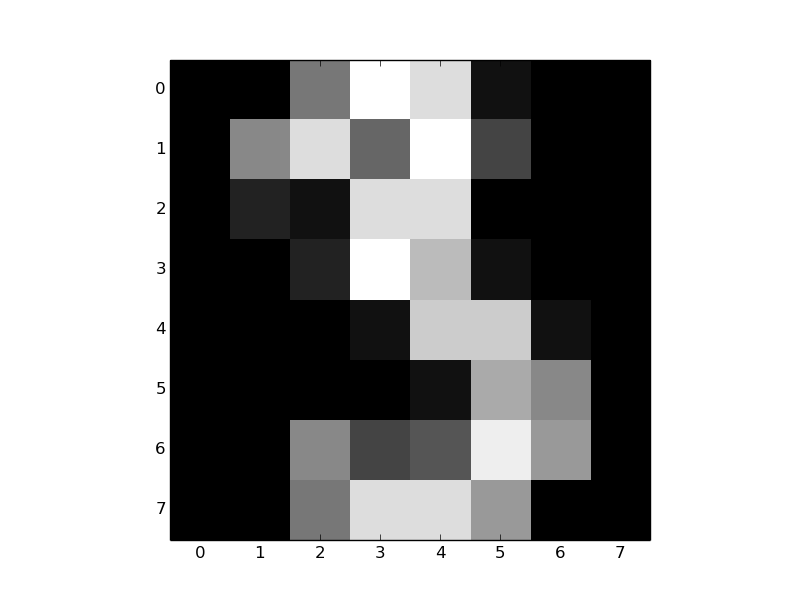
\includegraphics[width=0.33\textwidth]{task1.png}
	\caption{Digit 3}
	\label{fig1}
\end{figure}

\subsection{Nearest Neighbor Classifier}

The main aim of this exercise is to implement the k-Nearest Neighbor Classifier and apply it on the digit data set.

First step is to implement a function, that computes Euclidean distance between all digits in training and test set. We did it in two ways: the first implementation uses {\it for}-loops and the second uses advantages of vectorization. We explain shortly algorithms used in each function.

Assuming, $a_1,a_2,..a_{d_a}$ and $b_1,b_2,..b_{d_b}$ are respective our training and test images. Notice that each $a_i, b_j \in \mathbb{R}^{d}$, where $d$ is dimension  of the image space ($d=64$ in our case). To calculate the distance between $a_i$ and $b_j$ the first function uses the simple formula $dist(a_i,b_j) = \sqrt(a_i^2 - b_j^2)$ (see the code below).


\lstinputlisting[language=Python]{dist_loop.py}

To avoid slow loops we use a following vectorization in the second function:
\vspace*{12pt}
$dist(a_i,b_j) = \sqrt(a_i^2 - b_j^2) = a_i^2+b_j^2-2a_ib_j$ implies the following matrix form

$
dist(A,B) = 
\begin{bmatrix} 
	a_1^2 & a_1^2 & \cdots & a_1^2 \\
	a_2^2 & a_2^2 & \cdots & a_2^2 \\
	\vdots & \ddots & \vdots \\
	a_{d_a}^2 & a_{d_a}^2 & \cdots & a_{d_a}^2
\end{bmatrix}
+
\begin{bmatrix} 
	b_1^2 & b_2^2 & \cdots & b_{d_b}^2 \\
	b_1^2 & b_2^2 & \cdots & b_{d_b}^2 \\
	\vdots & \ddots & \vdots \\
	b_1^2 & b_2^2 & \cdots & b_{d_b}^2
\end{bmatrix}
-2
\left[ 
\begin{array}{c}
	 a_1\\ a_2 \\ \vdots \\ a_{d_a} \end{array} \right]
	 \times
	 \left[ \begin{array}{cccc} b_1 & b_2 & \cdots & b_{d_b} \end{array} \right] 
$

\vspace*{12pt}
\lstinputlisting[language=Python]{dist_vec.py}
\vspace*{12pt}
The running time of both function on the same training and data sets can be founded in the Table \ref{Tab1}.

\begin{table}[htb]
	\centering
	\begin{tabular}{|l | c|}
		\hline
		function & run time \\ \hline
		dist\_ loop & $9.78541$ sec \\ 
		dist\_ vec &  $0.02423$ sec\\ \hline 
	\end{tabular}
\caption{Running time of two distance functions}
\label{Tab1}
\end{table}

The complete k-Nearest Neighbor Classifier function uses the implemented distance function to find for each image from the test set it's k nearest neighbors in the training set. For $k>1$ the function collects the votes (classes of the neighbors) and picks the most common one.

\lstinputlisting[language=Python]{kNN.py}

Here are results of running the implemented kNN-Algorithm on the sets of the digits $1, 3$ and $1,7$ with different $k$ (see Table \ref{Tab2}).

\begin{table}[htb]
	\centering
	\begin{tabular}{|l|c|c|}
		\hline
		set & k & correct classification rate\\ \hline
		$1$ and $3$ & k=1 & $0.6$\\ \hline
		$1$ and $7$ & k=1 & $0.57931$\\ 
		$1$ and $7$ & k=3 & $0.61379$\\ 
		$1$ and $7$ & k=5 & $0.63448$\\ 
		$1$ and $7$ & k=9 & $0.67586$\\ 
		$1$ and $7$ & k=17 & $0.64827$ \\ 						
		$1$ and $7$ & k=33 & $0.65517$\\ \hline		
	\end{tabular}
\caption{Results of kNN-Classifier}
\label{Tab2}
\end{table}

We can see that increasing the number of neighbors results in better classification rate. The possible explanation might be that the higher $k$ makes algorithm robuster agains outliers. 

\subsection{Cross-Validation}
 In this part of the exercise we implement an n-fold cross validation scheme to test our k-Nearest Neighbors classifier.

To be able to do this we wrote function which splits our digit set in $n$ groups with equal number of elements in each group.
The function returns the indices of the corresponding images of the dataset in each of $n$ groups :
 
\lstinputlisting[language=Python]{split_dataset.py}

Each of $n$ groups will be used one time as a test set and the remaining parts as a training set. For each $n$ we calculate the mean classification rate and the variance. Results are shown in the table \ref{Tab3}.

\begin{table}[htb]
	\centering
	\begin{tabular}{|l|c|c|}
		\hline
		n & mean correct classification rate & variance\\ \hline
		n=1 & $0.113464$ & $7.93933868408e-05$\\ \hline
		n=5 & $0.116699$ & $0.00079345703125$\\ \hline
		n=10 & $0.106079101562$ & $0.000761985778809$\\ \hline		
	\end{tabular}
\caption{n-fold cross validation of kNN-Classifier, k = $1$}
\label{Tab3}
\end{table}


\section{Complete Code}

\lstinputlisting[language=Python]{../ex01.py}

\end{document}
%------------------------------------------------------------------------------%                                    
